\documentclass[12pt]{article}

\usepackage{fullpage}
\usepackage{graphicx}
\usepackage{caption}
\usepackage{subcaption}
\usepackage{float}

\begin{document}

\title{Wavelet Transform in 1 Dimension}
\author{Sayre Christenson, PHYS 6960}
\date{}

\maketitle


\begin{abstract}

The wavelet transforms of two similar signals show differences caused by discrete frequency changes in time.
Then, random noise on a linear function is filtered out and separately reconstructed.

\end{abstract}



\section*{Introduction}

The Fourier transform captures the frequency information of a signal, but loses time resolution.
To include time data in the analysis, the wavelet transform must be used.
The wavelet transform can be though of as a generalization of the Fourier transform concept, because instead of totally converting from time basis to frequency basis wavelet transforms result in a mix of time and frequency information.
Another way of explaining this is with the time-frequency uncertainty of signal processing, which states that a signal cannot be local in both time and frequency.
The Fourier transform has no temporal locality because it analyzes the entire signal at once, while the wavelet transform analyzes parts of the signal to describe some frequency information, mixing the locality of time and frequency.

A wavelet itself is a single oscillation (one requirement is that over one period the wavelet function integrates to 0) which plays the same role as a single sine or cosine oscillation in the Fourier transform.
Importantly, wavelets usually decay in intensity as their arguments approach infinity, which gives them a locality that differs from sines and cosines.
The wavelet transform also has a scaling component that picks up higher frequency signal components, usually corresponding to signal changes.
This scaling function picks up higher frequency information that is otherwise filtered out by the localized wavelet bandpass.

\section*{Daubechies 20 Wavelet Transform}

Using provided codes, 
Figures 1 and 2 show these signals and their wavelet transforms, 

\[
f_1(x) = \frac{1}{3}(\sin(2\pi x) + \sin(4\pi x) + \sin(5\pi x))
\]
\[
f_2(x) = \left\{
  \begin{array}{l l}
    \sin(2\pi x) & \quad \textrm{if} \; x \le \pi \\
    \sin(4\pi x) & \quad \textrm{if} \; \pi < x \le 2\pi \\
    \sin(5\pi x) & \quad \textrm{if} \; x > 2\pi 
  \end{array} \right.\]

and Figure 3 shows the wavelet decompression of a filtered signal.



\begin{figure}
  \centering

  \begin{subfigure}[b]{0.85\textwidth}
    \fbox{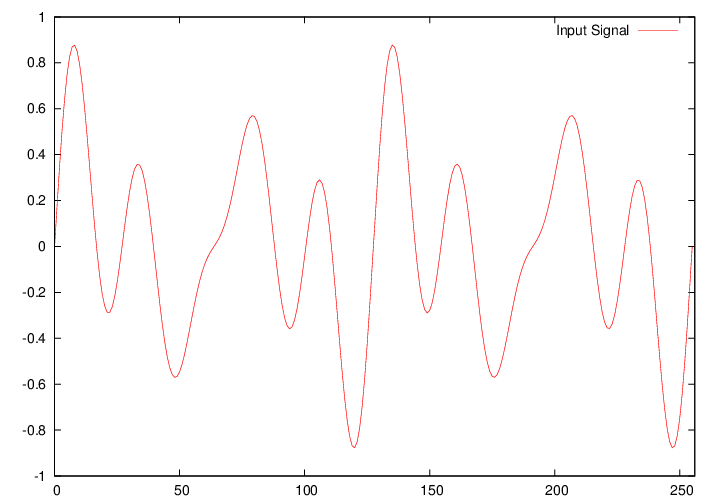
\includegraphics[width=1\textwidth]{orig1.png}}
    \caption{$f_1(x)$}
  \end{subfigure}
  \qquad
  \begin{subfigure}[b]{0.85\textwidth}
    \fbox{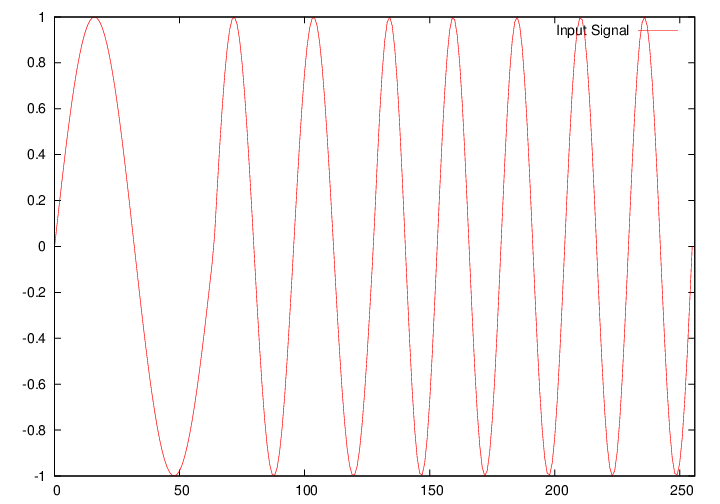
\includegraphics[width=1\textwidth]{orig2.png}}
    \caption{$f_2(x)$}
  \end{subfigure}

  \caption{Original Functions}
  \label{orig}

\end{figure}

\begin{figure}
  \centering

  \begin{subfigure}[b]{0.85\textwidth}
    \fbox{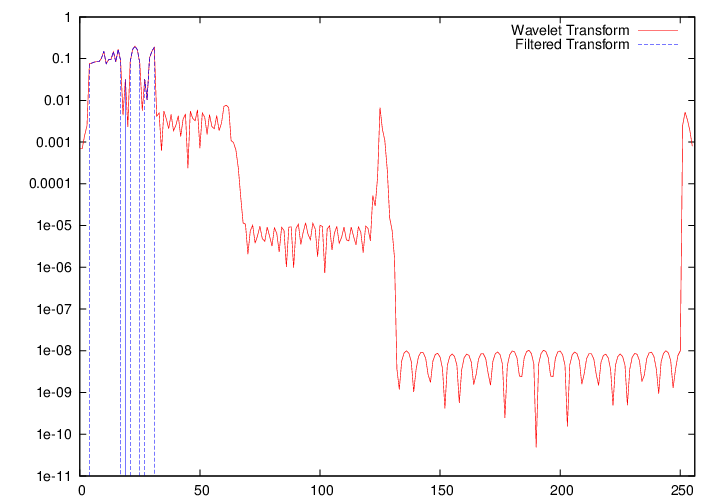
\includegraphics[width=1\textwidth]{wt1.png}}
    \caption{$f_1(x)$}
  \end{subfigure}
  \qquad
  \begin{subfigure}[b]{0.85\textwidth}
    \fbox{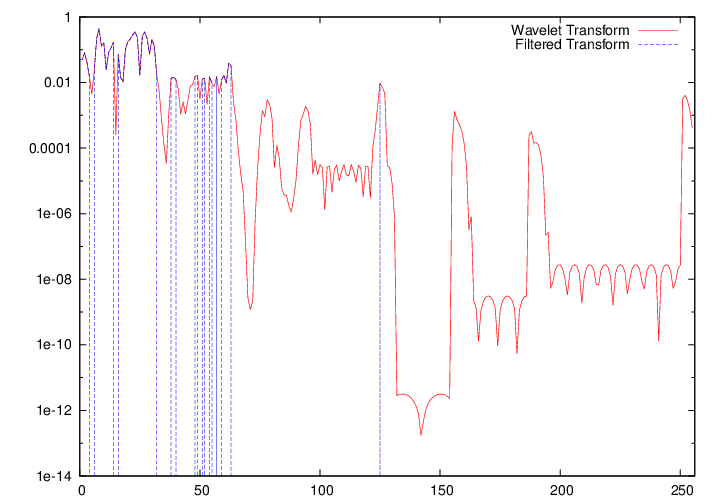
\includegraphics[width=1\textwidth]{wt2.png}}
    \caption{$f_2(x)$}
  \end{subfigure}

  \caption{Wavelet Transforms}
  \label{wt}

\end{figure}

\begin{figure}
  \centering

  \begin{subfigure}[b]{0.85\textwidth}
    \fbox{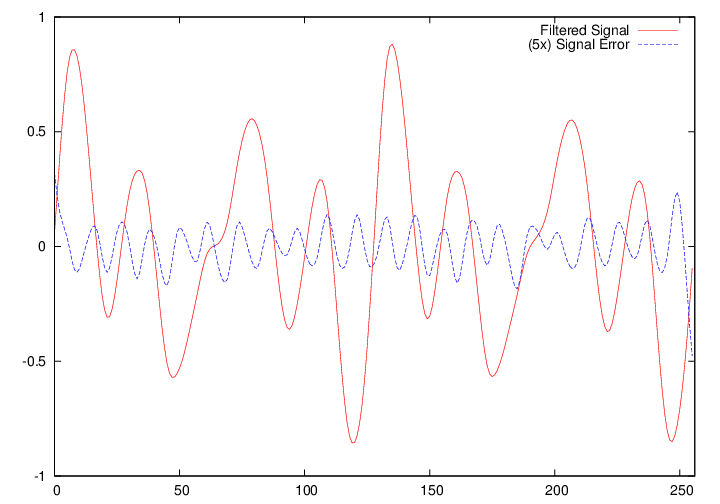
\includegraphics[width=1\textwidth]{revwt1.png}}
    \caption{$f_1(x)$}
  \end{subfigure}
  \qquad
  \begin{subfigure}[b]{0.85\textwidth}
    \fbox{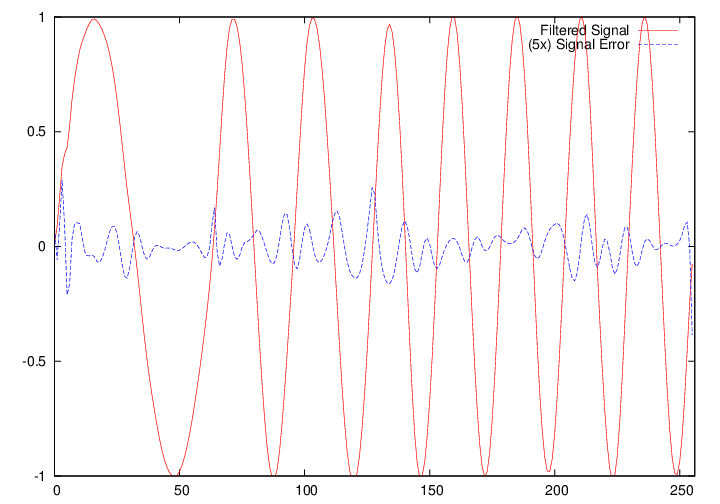
\includegraphics[width=1\textwidth]{revwt2.png}}
    \caption{$f_2(x)$}
  \end{subfigure}

  \caption{Inverse Wavelet Transform, Threshold = 0.1}
  \label{revwt}

\end{figure}

\end{document}
